% Metódy inžinierskej práce

\documentclass[10pt,oneside,english,a4paper]{article}

\usepackage[english]{babel}
%\usepackage[T1]{fontenc}
\usepackage[IL2]{fontenc} % lepšia sadzba písmena Ľ než v T1
\usepackage[utf8]{inputenc}
\usepackage{graphicx}
\usepackage{background}
\usepackage{booktabs} 
\usepackage{caption} 
\usepackage{subcaption} 
\usepackage{multicol}
\usepackage{amsmath, amssymb}
\usepackage{array, hhline}
\usepackage{cite}
\usepackage[normalem]{ulem}
\usepackage{comment}
\usepackage{url} % príkaz \url na formátovanie URL
\usepackage{hyperref} % odkazy v texte budú aktívne (pri niektorých triedach dokumentov spôsobuje posun textu)
\usepackage{everypage}

%\usepackage{times}

%logo
\backgroundsetup{
    contents=
\includegraphics{STU-FIIT.png},
    scale=0.3,
    opacity=1,
    angle=0,
    position=current page.north,
    vshift=-4cm
}

\pagestyle{headings}

\title{Real-time data processing in autonomous vehicles\thanks{Semestrálny projekt v predmete Metódy inžinierskej práce, ak. rok 2023/24, vedenie: Pavol Baťalík}} % meno a priezvisko vyučujúceho na cvičeniach

\author{Maksim Alehash\\[2pt]
	{\small Slovenská technická univerzita v Bratislave}\\
	{\small Fakulta informatiky a informačných technológií}\\
	{\small \texttt{xalehash@stuba.sk}}
	}

\date{\small\today} % upravte



\begin{document}

\maketitle

\begin{abstract}
The astounding leaps in AI technology have made autonomous vehicles the sole means of modern transportation, placing an emphasis on enhancing a person's safety, adapting to the comfort of the passengers, and making the ride as efficient as possible. In order to get the best results in the shortest amount of time possible, the machines need to make split-second decisions in order to achieve them. 
\par The article presents a comprehensive exploration of the critical role of real-time data processing, which is one of the most crucial parts of autonomous vehicles. It covers the essence and the functioning of many cutting-edge technologies and methods that are being used, how the data is being processed in general and touches on the safety and unparalleled comforts whilst driving, but also the risks and challenges it can pose. In the end, the article illustrates to readers the intricacies and implications of real-time data processing that play a crucial role in autonomous vehicles.
\end{abstract}


\tableofcontents\pagebreak 


\section{Introduction} \label{introduction}

Motivujte čitateľa a vysvetlite, o čom píšete. Úvod sa väčšinou nedelí na časti.

Uveďte explicitne štruktúru článku. Tu je nejaký príklad.
Základný problém, ktorý bol naznačený v úvode, je podrobnejšie vysvetlený v časti~\ref{}.
Dôležité súvislosti sú uvedené v častiach~\ref{dolezita} a~\ref{dolezitejsia}.
Záverečné poznámky prináša časť~\ref{zaver}.



\section{Sensors and data sources} \label{sensors and data sources}

Z obr.~\ref{f:rozhod} je všetko jasné. 

\begin{figure*}
%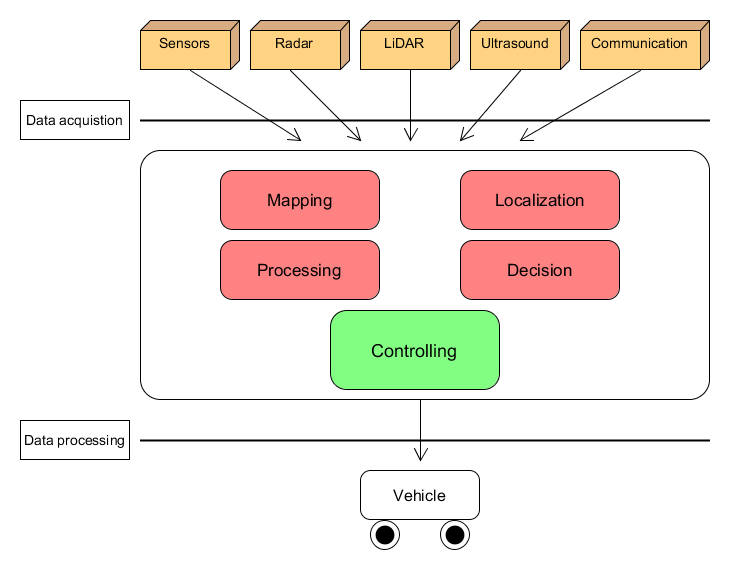
\includegraphics[scale=1.0]{diagram.pdf}
Aj text môže byť prezentovaný ako obrázok. Stane sa z neho označný plávajúci objekt. Po vytvorení diagramu zrušte znak. pred príkazom \verb|\includegraphics| označte tento riadok ako komentár (tiež pomocou znaku ).


\centering
    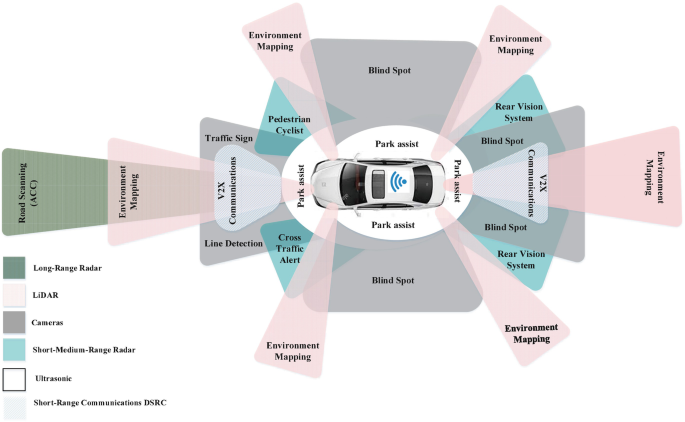
\includegraphics[width=10cm]{sensors.png}
    \caption\centering{The complexity situation awareness of autonomous vehicle caused by using multi-sensors}
    \label{fig:sensors}
    
\end{figure*}

\section{Data processing architecture} \label{architecture}

Základným problémom je teda\ldots{} Najprv sa pozrieme na nejaké vysvetlenie (časť~\ref{ina:nejake}), a potom na ešte nejaké (časť~\ref{ina:nejake}).\footnote{Niekedy môžete potrebovať aj poznámku pod čiarou.}

Môže sa zdať, že problém vlastne nejestvuje\cite{Coplien:MPD}, ale bolo dokázané, že to tak nie je~\cite{Czarnecki:Staged, Czarnecki:Progress}. Napriek tomu, aj dnes na webe narazíme na všelijaké pochybné názory\cite{PLP-Framework}. Dôležité veci možno \emph{zdôrazniť kurzívou}.

\begin{figure*}


\centering
    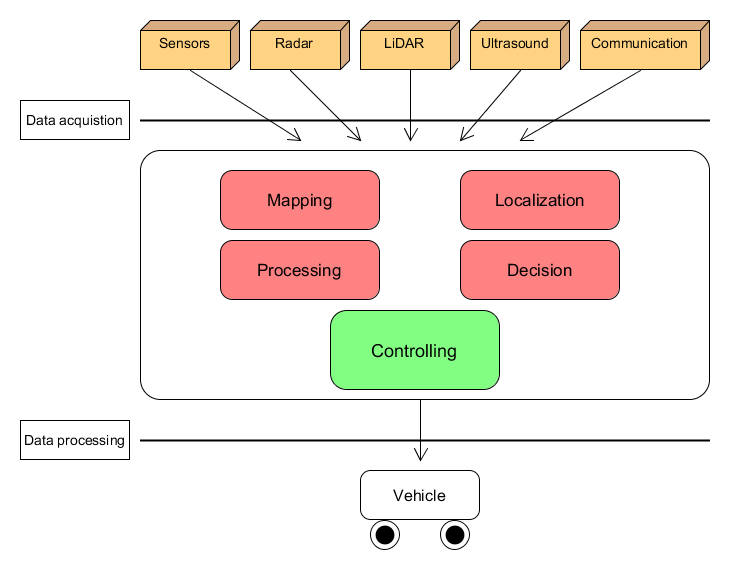
\includegraphics[width=10cm]{architecture.png}
    \caption{Architecture}
    \label{fig:architecture}

\end{figure*}

\section{Algorithms and methods} \label{dolezita}



\[Matica
\begin{bmatrix}
1 & 2 & 3 & 4 & 5\\
1 & 2 & 3 & 4 & 5\\
1 & 2 & 3 & 4 & 5\\
1 & 2 & 3 & 4 & 5\\
1 & 2 & 3 & 4 & 5\\
\end{bmatrix}
\]

Postupnost
\begin{align}
    F(x) &= a_0 + a_1 x + a_2 x^2 + a_3 x^3 + a_4 x^4 \nonumber \\
         &\quad + a_5 x^5 + a_6 x^6 + a_7 x^7 + a_8 x^8 \nonumber \\
         &\quad + a_9 x^9 + a_{10} x^{10} + a_{11} x^{11} \nonumber
\end{align}

\section{Safety and performance} \label{dolezitejsia}




\section{Future directions and challenges} \label{dolezitejsia}

Nieco \cite{8501581}
\cite{8457076}
\cite{9214125}
\cite{Khayyam2020}
\cite{8679433}
\cite{8809661}
\cite{YOGANANDHAN20203303}
\cite{electronics12153223}
\cite{s23063335}
\cite{9288755}


\section{Conclusion} \label{zaver} % prípadne iný variant názvu



%\acknowledgement{Ak niekomu chcete poďakovať\ldots}


% týmto sa generuje zoznam literatúry z obsahu súboru literatura.bib podľa toho, na čo sa v článku odkazujete
\newpage
\bibliography{literatura}
\bibliographystyle{unsrt} % prípadne alpha, abbrv alebo hociktorý iný
\end{document}

\begin{comment}
\cite{8501581}
\cite{8457076}
\cite{9214125}
\cite{Khayyam2020}
\cite{8809661}
\cite{YOGANANDHAN20203303}
\cite{electronics12153223}
\cite{s23063335}
\cite{9288755}
\cite{7368032}
\cite{8809661}
\end{comment}


